\lecture{Adders and Subtractors}{25-10-22}{16:00}{Farzad}{RB LT1}

Within computers, there needs to be a way that numbers can be added together and subtracted. This is done using something called an adder subtractor. There are a number of different versions of the circuit which we need to look at first. 

\section*{Half Adder}
To start with, if we look at a truth table showing two inputs ($B$ and $A$) and two outputs ($sum$ and $carry$), we can show the combinations of gates which we need for a half adder. 
\begin{table}[H]
    \centering
    \begin{tabularx}{0.35\textwidth}{XX|XX}
        B & A & sum & carry\\
        \hline
        0 & 0 & 0 & 0\\
        0 & 1 & 1 & 0\\
        1 & 0 & 1 & 0\\
        1 & 1 & 0 & 1\\
    \end{tabularx}
\end{table}
From the table, we can see that the sum column represents the truth table for an XOR gate and the carry column represents the truth table for an AND gate. We can draw this as a circuit diagram.
\begin{center}
\begin{circuit}
    \node[] (A) at (0,2.25) {A};
    \node[] (B) at (0,1.75) {B};
    \node[xor port] (xor) at (3,2) {};
    \node[and port] (and) at (3,0) {};

    \draw(A.east) |- (xor.in 1);
    \draw(B.east) |- (xor.in 2);
    \draw(xor.in 1) ++(-0.4, 0) |- (and.in 1);
    \draw(xor.in 2) ++(-0.7, 0) |- (and.in 2);
    \draw(xor.out) -- ++(0.5,0) node[right] {Sum};
    \draw(and.out) -- ++(0.5,0) node[right] {Carry};
\end{circuit}
\end{center}
\section*{Full Adder}
The circuit above is all well and good for adding one bit to another bit, but what if we are trying to do two bit addition (e.g. 11 + 01). The table below shows how we would express this in a truth table.
\begin{table}[H]
    \centering
    \begin{tabularx}{0.4\textwidth}{XXX|XX}
        A & B & C$_{in}$ & sum & C$_{out}$\\
        \hline
        0 & 0 & 0 & 0 & 0 \\
        0 & 0 & 1 & 1 & 0 \\
        0 & 1 & 0 & 1 & 0 \\
        0 & 1 & 1 & 0 & 1 \\
        1 & 0 & 0 & 1 & 0 \\
        1 & 0 & 1 & 0 & 1 \\
        1 & 1 & 0 & 0 & 1 \\
        1 & 1 & 1 & 1 & 1 \\
    \end{tabularx}
\end{table}
This addition is a two stage. First add $A+B = S_{interim}+C_{interim}$. Then add $C_{in + S} = S_{out} + C_{interim2}$. This can be represented in the following circuit.
\begin{figure}[H]
    \centering
    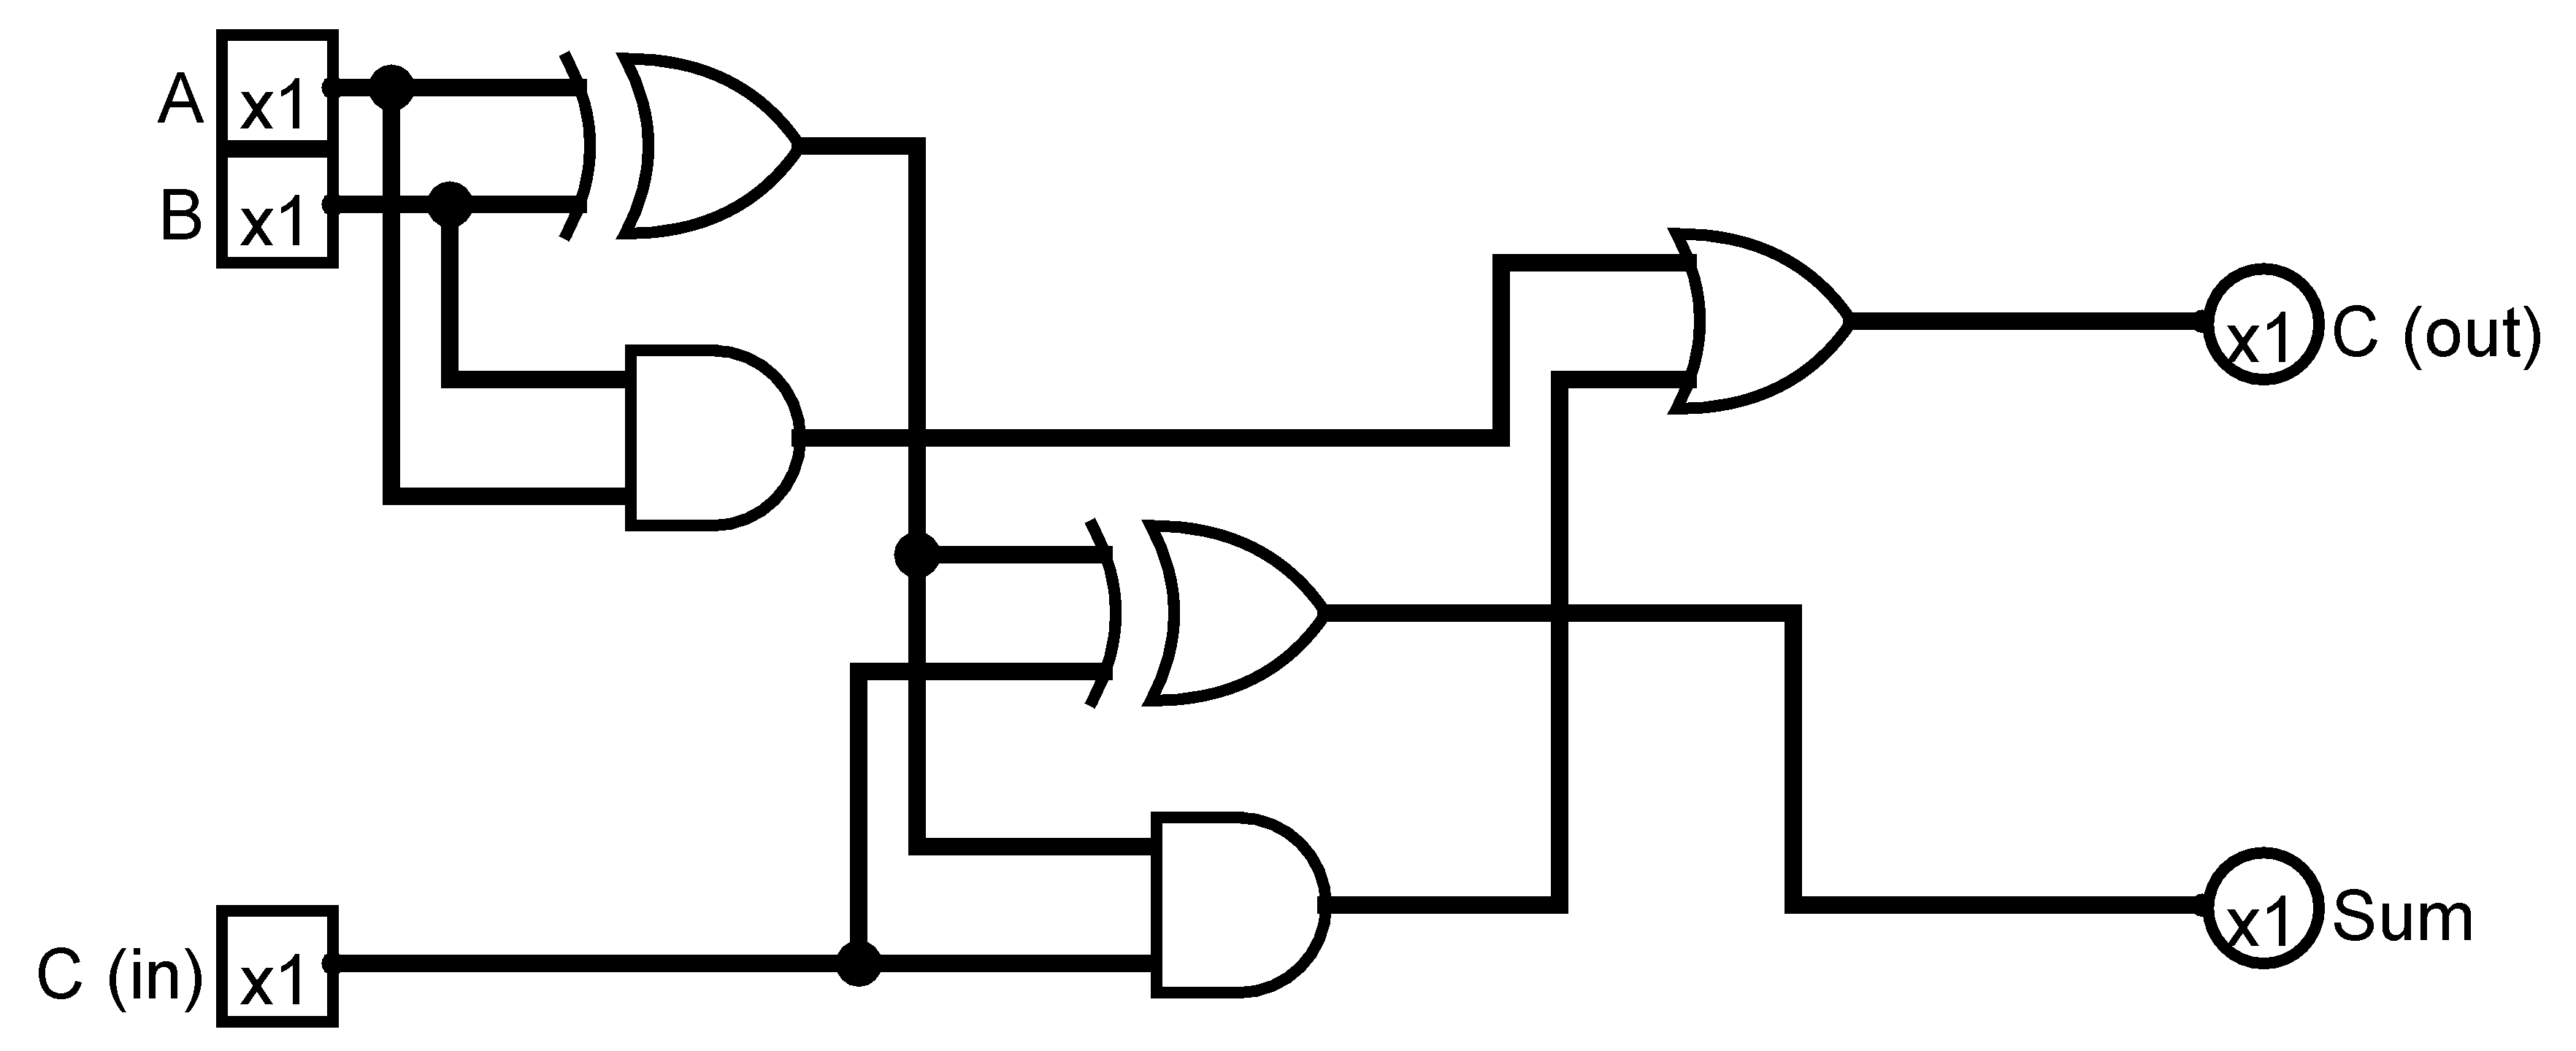
\includegraphics[width=0.8\textwidth]{assets/full-adder-img.png}
\end{figure}
We can turn this circuit into a block for diagram simplicity.
\begin{figure}[H]
    \centering
    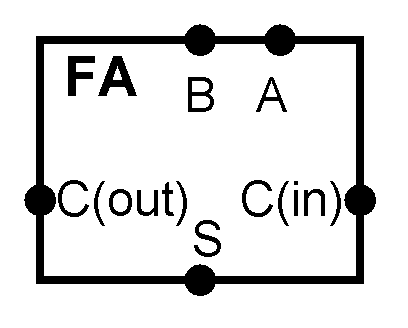
\includegraphics[width=0.2\textwidth]{assets/full-adder-block-img.png}
\end{figure}

So, using 5 gates we can add 2 bits and give a carry out (this is 2 XOR, 2 AND and 1 OR). What happens if we want to add 1101 and 0110 (4 bits).\\
We will need a bigger adder. The general rule of thumb is one full adder for each bit we want to add.
\begin{figure}[H]
    \centering
    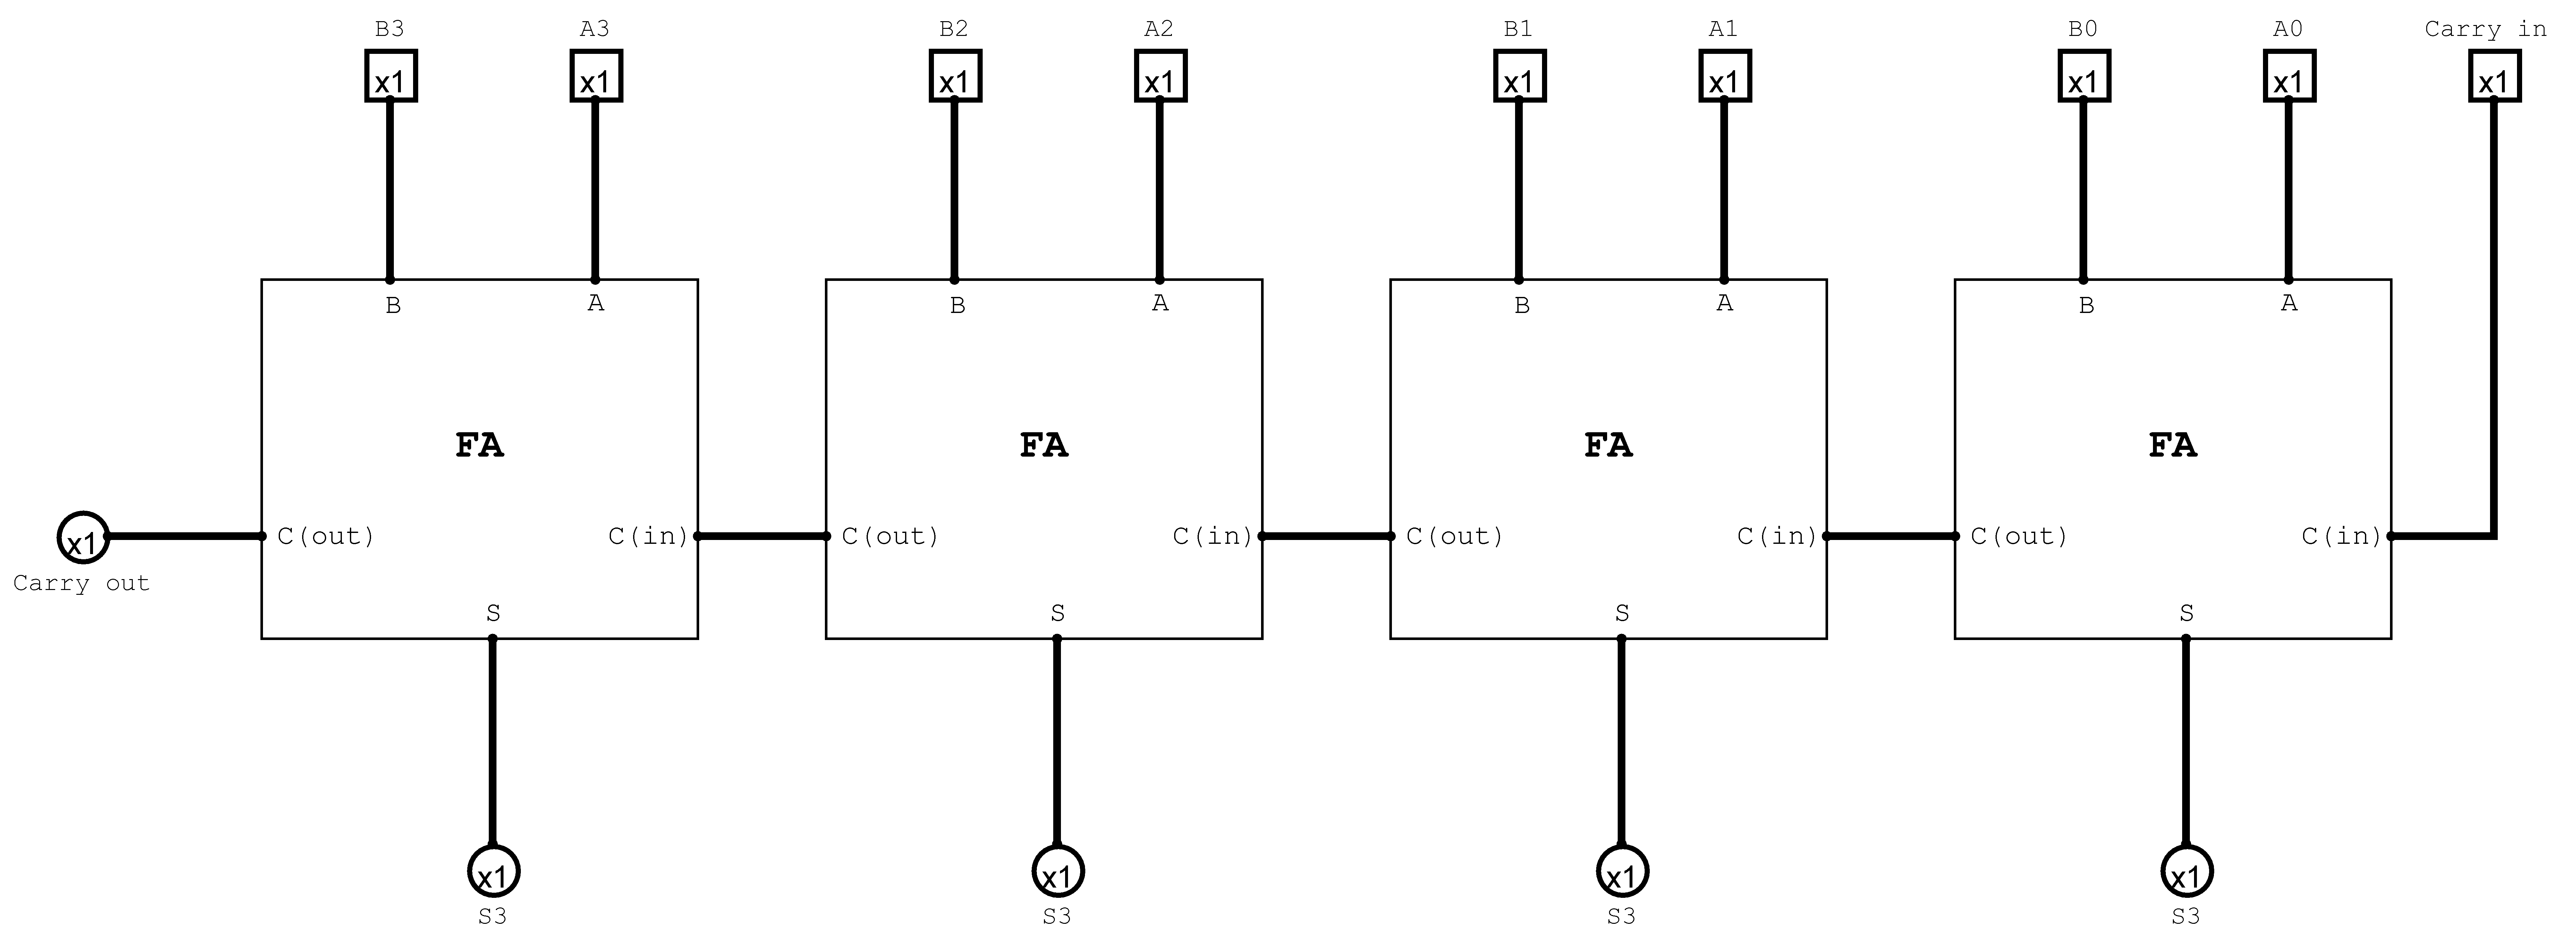
\includegraphics[width=0.8\textwidth]{assets/full-adder-4-bit.png}
\end{figure}

\section*{Subtracting}
As we know from earlier weeks, computers do not subtract, they add a negative number. This poses a challenge as we need to convert the second number in the sum to a negative number using a two's complement number. To do this, we have to first flip the bits then add a 1 to the cary in of the least significant bit adder. This would generate the following circuit diagram.
\begin{figure}[H]
    \centering
    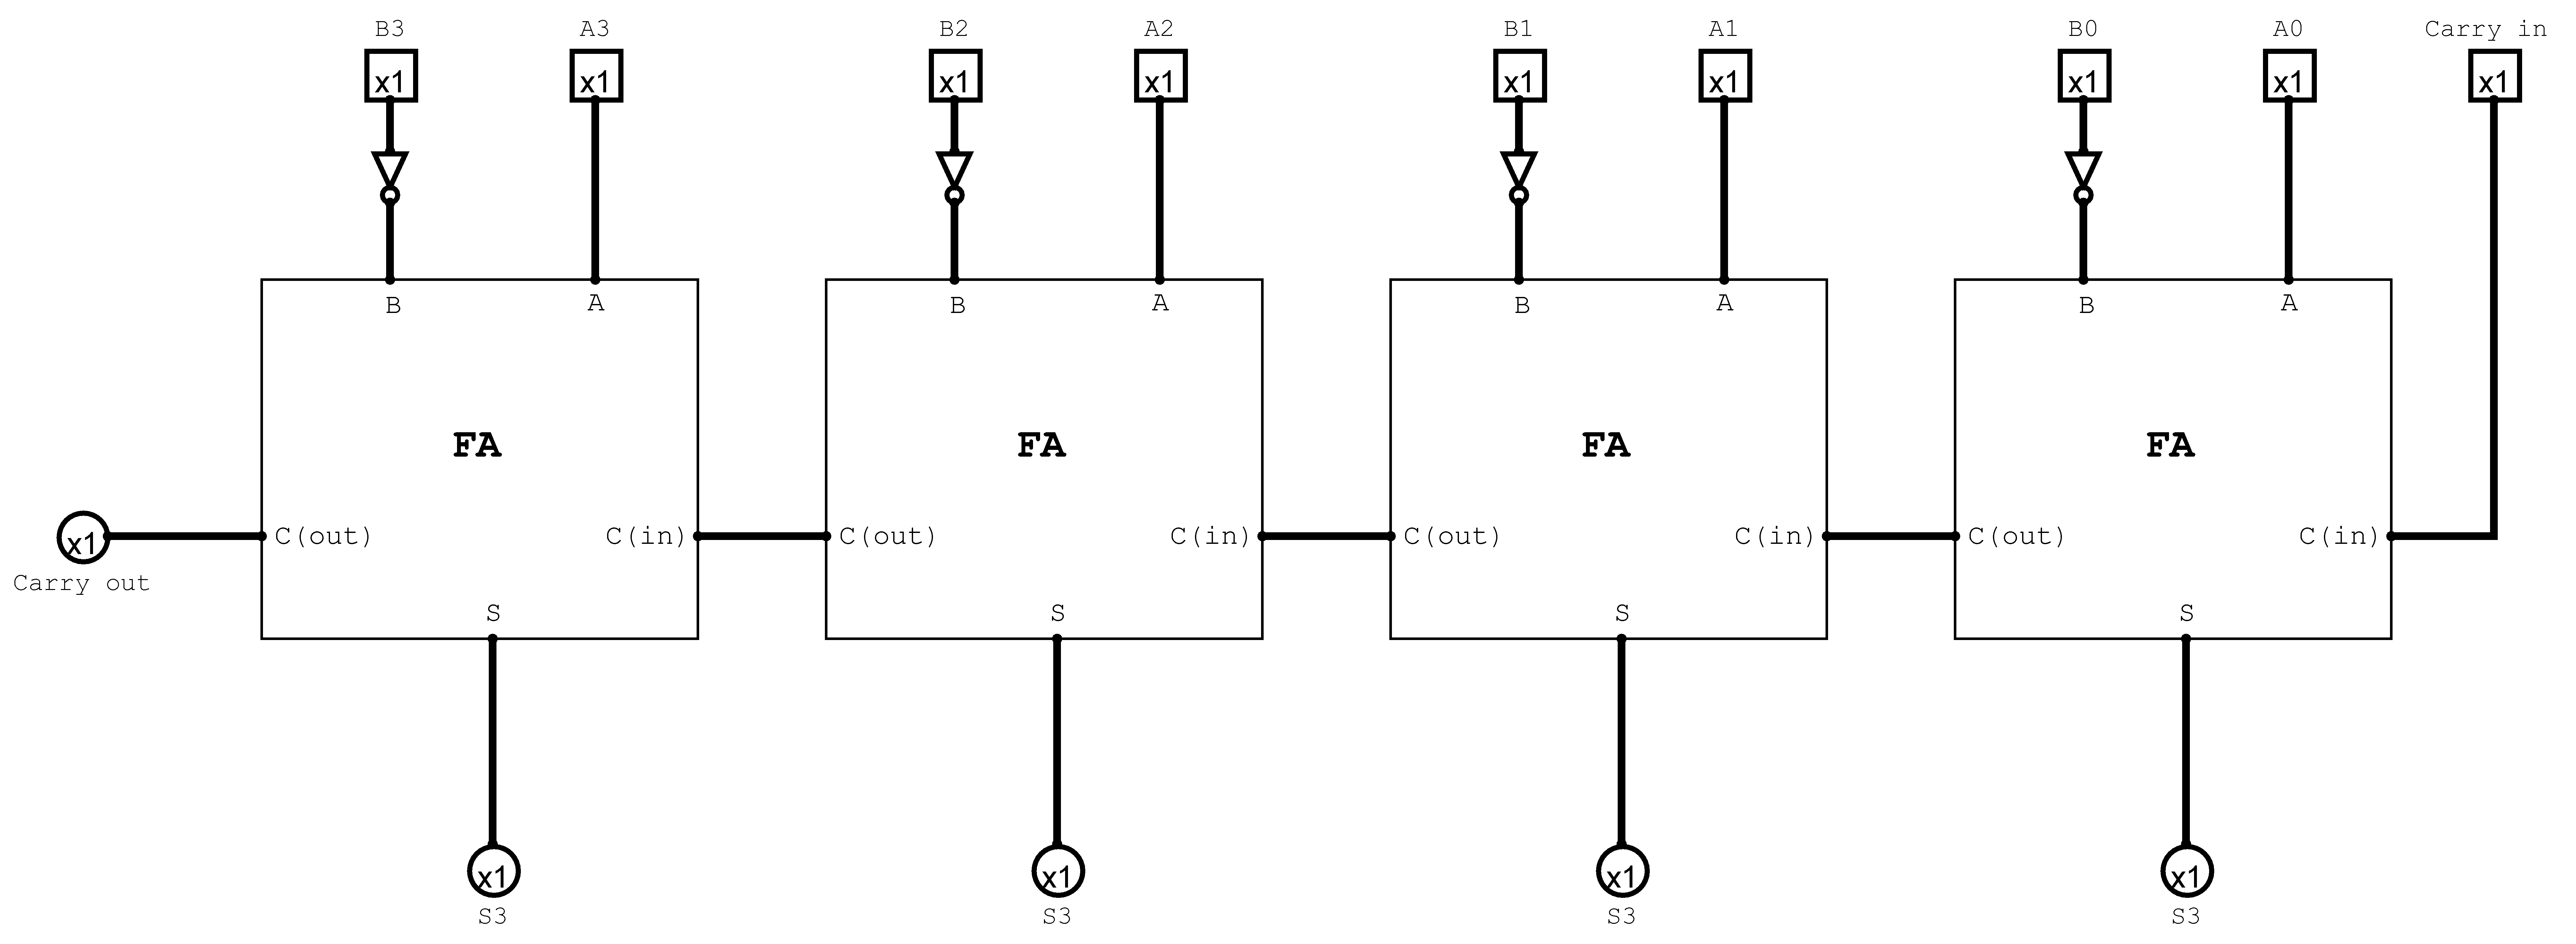
\includegraphics[width=0.8\textwidth]{assets/subtractor.png}
\end{figure}

We use two's complement to avoid having positive and negative zero.

Inside a computer, it is a bad use of space to have two circuits, we instead want one `General Purpose Circuit'. This should add and subtract.

\section*{Adder Subtractor}
The subtractor bit of the circuit will always flip B. We need to find a combination of gates that when set to add, doesn't invert and when set to subtract, it inverts B.  This gate is the XOR gate, this circuit diagram is shown below.
\begin{figure}[H]
    \centering
    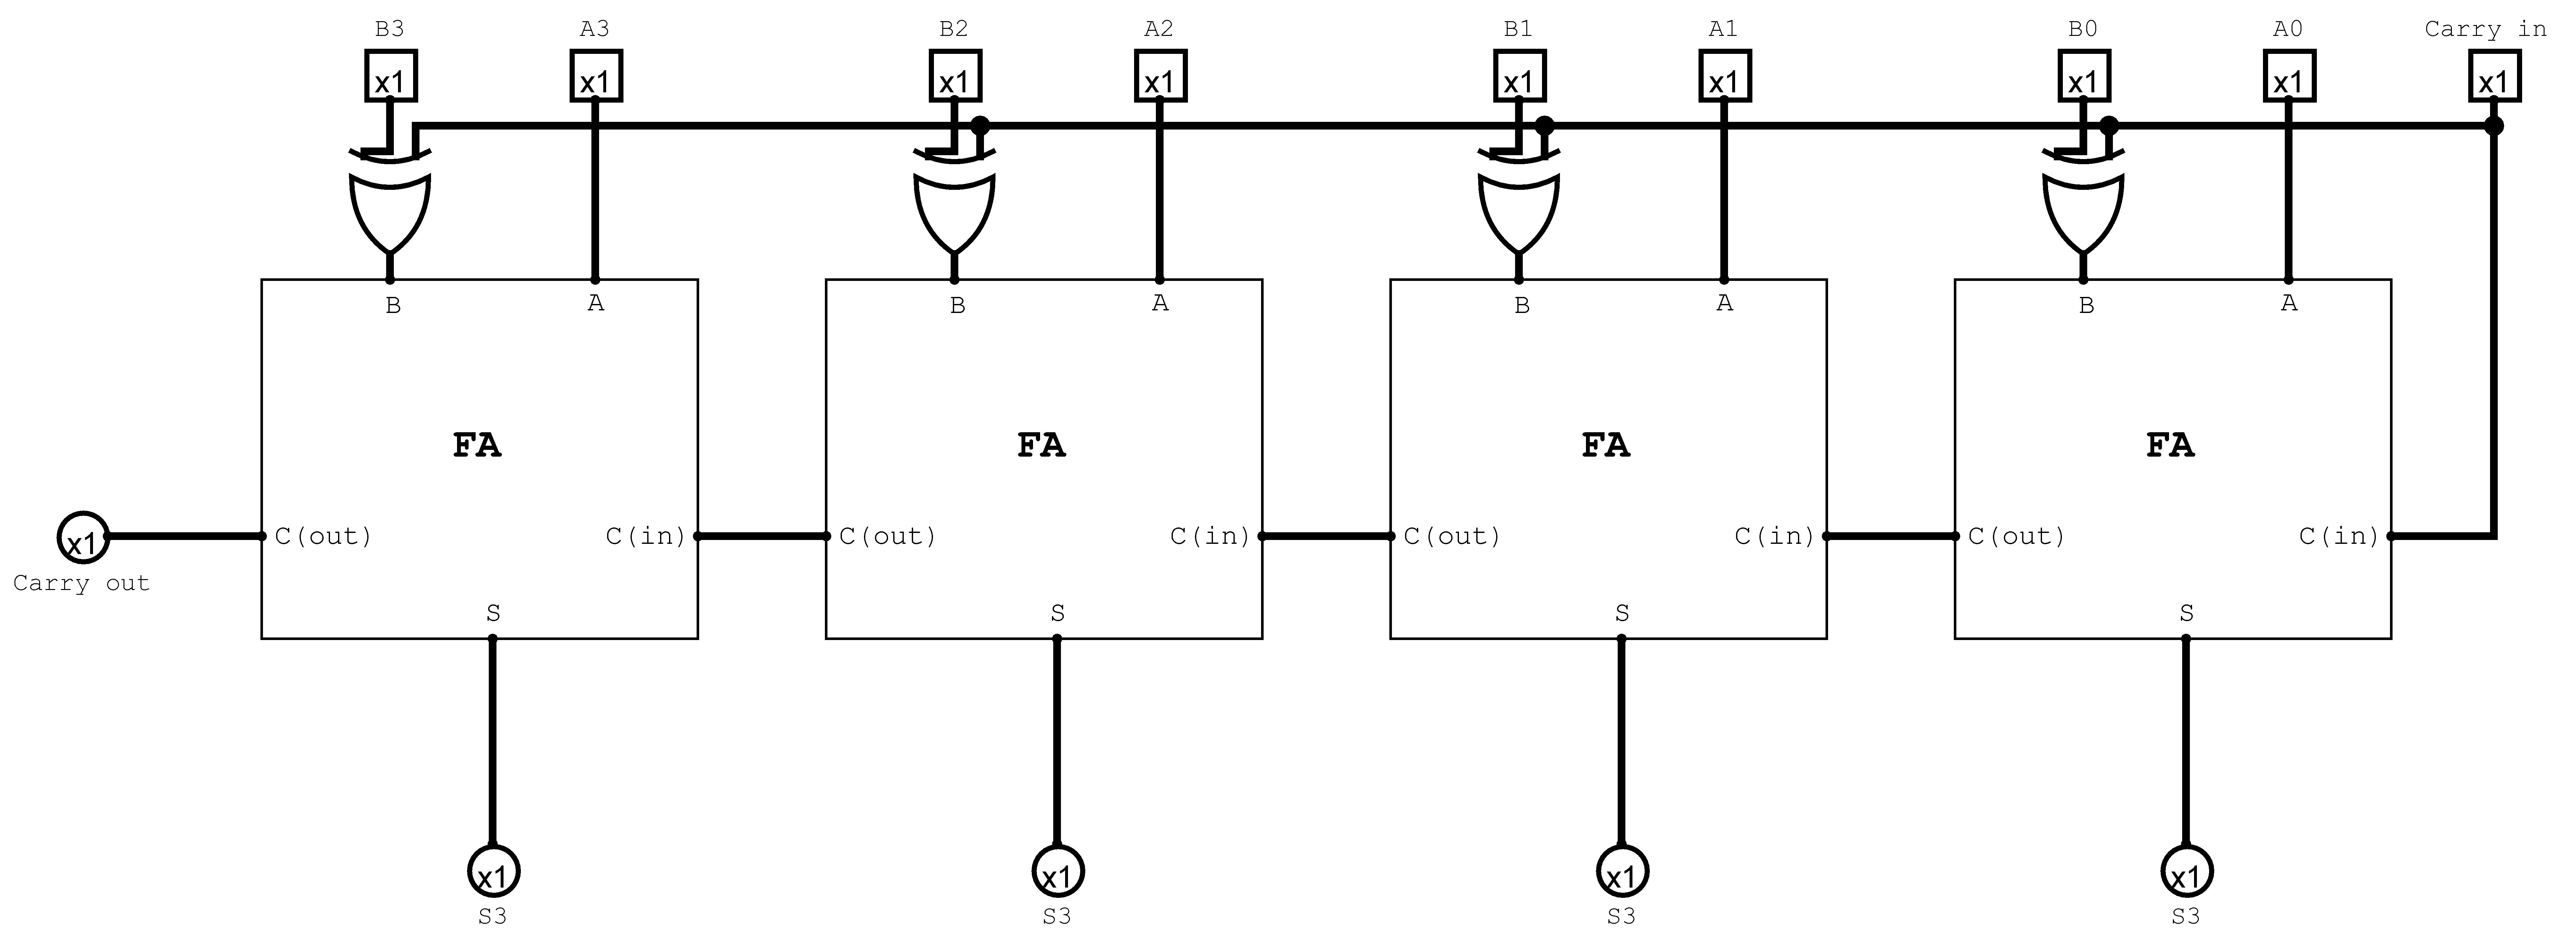
\includegraphics[width=0.8\textwidth]{assets/add-subt.png}
\end{figure}

If the cary in switch is 0, $B$ is kept the same and $C_{in}=0$. If the carry in switch is 1, $B$ is flipped $=\overline{B}$ and $C_{in} = 1$, which adds the 1 needed for the addition part of two's complement.